\begin{table}[t!]
    \begin{minipage}{0.5\columnwidth}
        
        \centering
        \caption{\textbf{Additional ablation study of training objectives and learning stages on robot manipulation benchmarks.}}
        \label{tab:supp:ablation_stage_loss}
    
        \centering
        \resizebox{\linewidth}{!}{
        \begin{tabular}{lcccc}
            \toprule
            \makecell{\textbf{Method}} &
            \makecell{\textbf{LIBERO}} &
            \makecell{\textbf{SimplerEnv}\\\textbf{Google}} &
            \makecell{\textbf{RoboTwin2.0}} &
            \makecell{\textbf{Average}} \\
            \midrule
            \textbf{Fast-ThinkAct} & \textbf{89.7} & \textbf{68.7} & \textbf{46.1} & \textbf{68.2} \\
            \midrule
            w/o $\mathcal{L}_\text{verb}$ & 88.6 & 67.3 & 44.9 & 66.9 \\
            w/o $\mathcal{L}_\text{verb},\mathcal{L}_\text{distill}$ & 86.3 & 65.7 & 42.6 & 64.9 \\
            \midrule
            Textual Teacher & 88.5 & 67.3 & 45.8 & 67.2 \\
            SFT + CoT-SFT & 87.2 & 65.8 & 43.3 & 65.4 \\
            SFT only & 86.9 & 64.5 & 42.8 & 64.7 \\
            \bottomrule
        \end{tabular}
    }

    \end{minipage}\hfill
    \begin{minipage}{0.46\columnwidth}

        \centering
        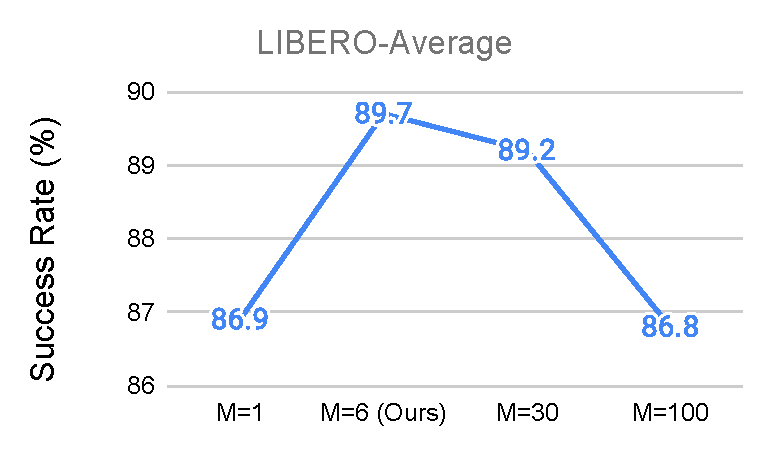
\includegraphics[width=\linewidth]{figures/images/supp_ablate_steps.pdf}

        \caption{\textbf{Ablation of Latent Reasoning Steps $M$.}}
    \label{fig:supp:ablate_steps}
    \end{minipage}

\end{table}
